\chapter{Исследовательский раздел}

\section{Технические характеристики}
Технические характеристики, используемого устройства:
\begin{itemize}
    \item[---] Операционная система --- Ubuntu Linux x86\_64~\cite{Ubuntu};
    \item[---] Память --- 16 Гб;
    \item[---] Процессор --- AMD Ryzen 5 5500U (6x2.10 ГГц)~\cite{AMD}.
\end{itemize}

\section{Оценка алгоритмов}
В данном разделе оценку трудоемкости алгоритма будем делать по количеству числа сравнений, понадобившихся для нахождения заданного элемента. Размер массива равен 1013.

В алгоритме линейного поиска количество возможных исходов равно длине массива: это $n$ вариантов, если элемент присутствует в множестве, плюс еще один исход, когда элемент отсутствует. В худшем случае число сравнений составит $n$. Наихудший сценарий возникает, когда элемент либо отсутствует, либо находится в самом конце массива. Линейный поиск на отсортированном множестве работает быстрее, если индекс искомого элемента меньше приблизительно, чем $\log_2(n)$. На рисунке~\ref{fig:Gist_Liniar} показана гистограмма работы данного алгоритма.

\begin{figure}[h]
	\centering
	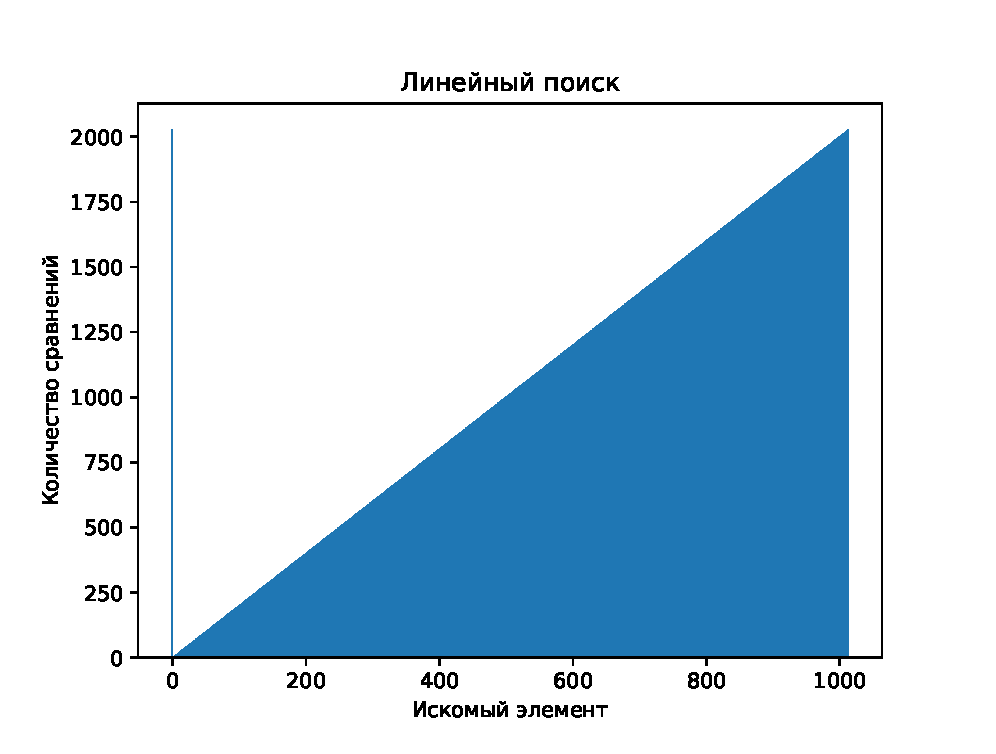
\includegraphics[]{img/Figure_1.eps}
	\caption{Гистограмма алгоритма линейного поиска}
	\label{fig:Gist_Liniar}
\end{figure}

\clearpage

В алгоритме двоичного поиска максимальное количество сравнений в худшем случае не превышает $\log_2(n)$. На рисунках~\ref{fig:Gist_Binary} и~\ref{fig:Gist_Binary_Sort} представлены гистограммы для этого алгоритма, при этом рисунок~\ref{fig:Gist_Binary_Sort} демонстрирует график, где количество сравнений отсортировано по возрастанию.

\begin{figure}[h]
    \centering
    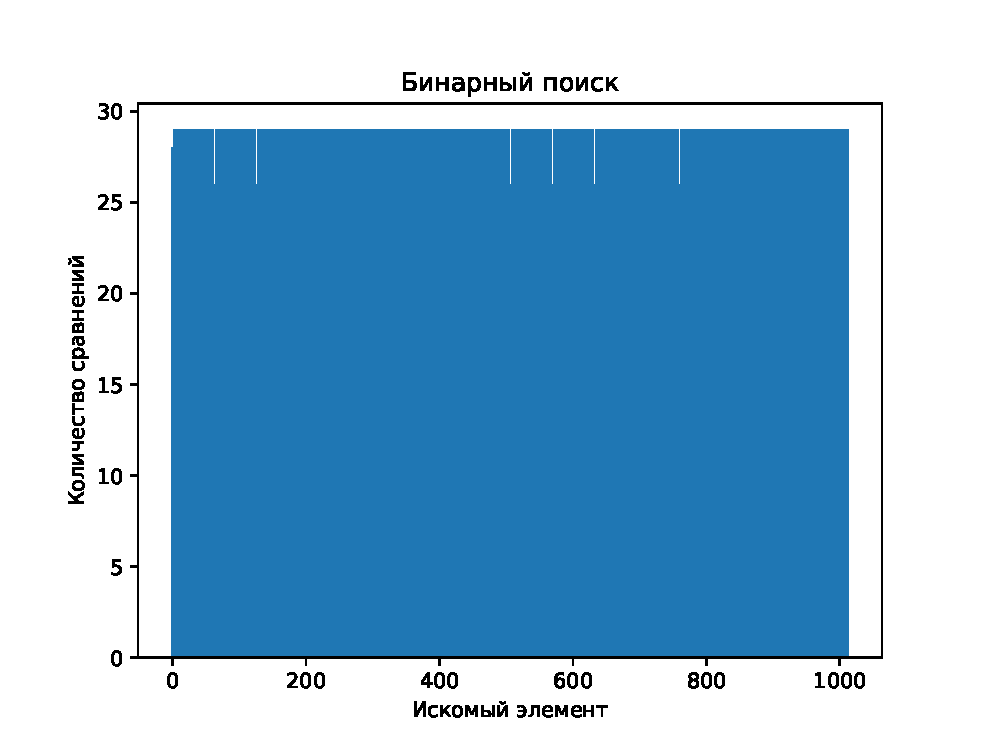
\includegraphics[scale=1]{img/Figure_2.eps}
    \caption{Гистограмма алгоритма с двоичным поиском}
    \label{fig:Gist_Binary}
\end{figure}

\clearpage
\begin{figure}[h]
    \centering
    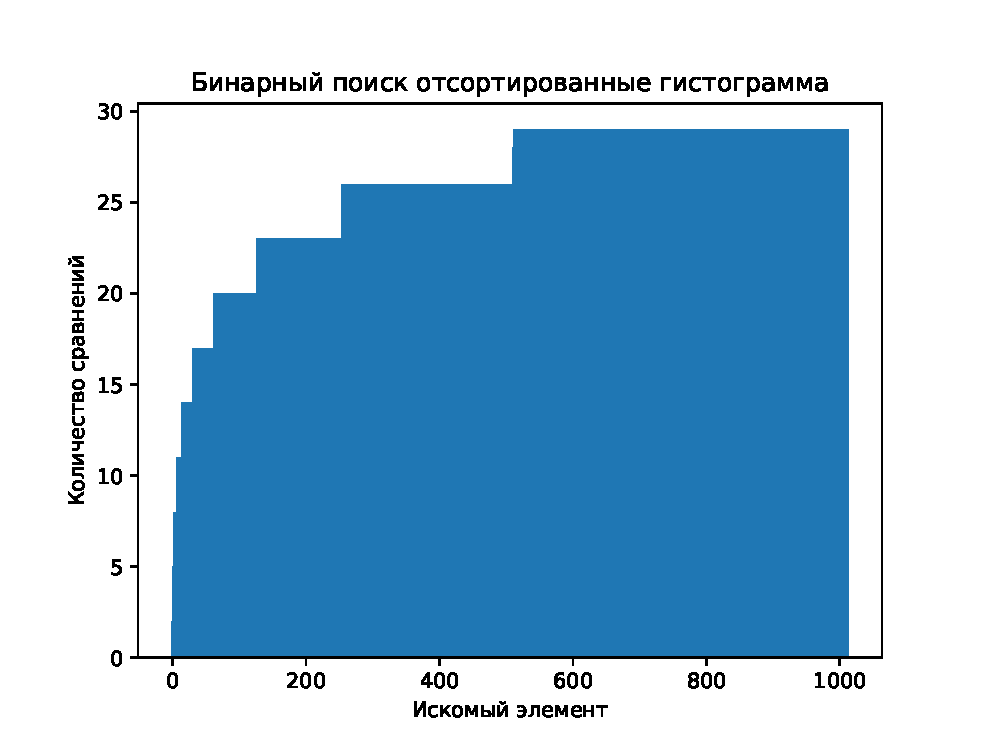
\includegraphics[width=0.8\textwidth]{img/Figure_3.eps}
    \caption{Гистограмма алгоритма с двоичным поиском, отсортированная по количеству сравнений}
    \label{fig:Gist_Binary_Sort}
\end{figure}

\clearpage
\section{Вывод}

При линейном поиске количество сравнений постепенно увеличивается с ростом индекса искомого элемента. Для двоичного поиска количество сравнений, в целом, не зависит от расположения элемента относительно начала или конца массива, хотя элементы, находящиеся ближе к середине массива, будут найдены быстрее. В некоторых случаях линейный поиск может оказаться быстрее бинарного на отсортированном множестве, если искомое значение имеет индекс, меньший, чем $\log_2(n)$. Например, для массива из 1013 элементов линейный поиск будет эффективнее на индексах от 1 до 12. 

В целом, двоичный поиск является более эффективным, поскольку в худшем случае требует не более $\log_2(n)$ сравнений, тогда как для полного перебора это значение составляет $n$.






